\section{Introduction}
\label{sec:intro}

Semantic segmentation is a core problem in computer vision, with the aim of partitioning an image into coherent regions with their respective semantic class labels. Most existing methods for semantic segmentation assume a limited set of semantic class labels that can potentially be assigned to a pixel. The number of class labels is dictated by the training dataset and typically ranges from tens \citep{Everingham15} to hundreds \citep{zhou2019semantic,mottaghi14} of distinct categories. As the English language defines several hundred thousand nouns \citep{li2020fss}, it is likely that the limited size of the label set severely hinders the potential recognition performance of existing semantic segmentation models.


The main reason for the restricted label sets in existing methods is the cost of annotating images to produce sufficient training data. To create training datasets, human annotators must associate every single pixel in thousands of images with a semantic class label -- a task that is extremely labor intensive and costly even with small label sets. The complexity of the annotation rises significantly as the number of labels increases since the human annotator has to be aware of the fine-grained candidate labels. Additionally, inter-annotator consistency becomes an issue when objects are present in an image that could fit multiple different descriptions or are subject to a hierarchy of labels.

Zero- and few-shot semantic segmentation methods have been proposed as a potential remedy for this problem.
Few-shot approaches~\citep{shaban2017one,rakelly2018conditional,siam2019amp,wang2019panet,zhang2019pyramid,nguyen2019feature,liu2020part,wang2020few,tian2020prior,boudiaf2021few,min2021hypercorrelation} offer ways to learn to segment novel classes based on only a few labeled images. However, these approaches still require labeled data that includes the novel classes in order to facilitate transfer. 
Zero-shot methods, on the other hand, commonly leverage word embeddings to discover or generate related features between seen and unseen classes~\citep{bucher2019zero,Gu2020CaGNet} without the need for additional annotations. Existing works in this space use standard word embeddings~\citep{word2vec} and focus on the image encoder.

In this work, we present a simple approach to leveraging modern language models to increase the flexibility and generality of semantic segmentation models. Our work is inspired by the CLIP model for image classification~\citep{radford2021learning}, which pairs high-capacity image and text encoders to produce robust zero-shot classifiers. We propose to use state-of-the-art text encoders that have been co-trained on visual data, such as CLIP, to embed labels from the training set into an embedding space and to train a visual encoder to produce per-pixel embeddings from an input image that are close to the corresponding label embeddings. Since the text encoder is trained to embed closely related concepts near one another (for example, ``dog'' is closer to 
``pet'' than to ``vehicle''), we can transfer the flexibility of the text encoder to the visual recognition module while only training on the restricted label sets that are provided by existing semantic segmentation datasets. An example is shown in Figure~\ref{fig:method_exp1} (top row), where the model can successfully label pixels belonging to the class ``pet'' although the training set did not contain this label.
\begin{figure}
    \centering
     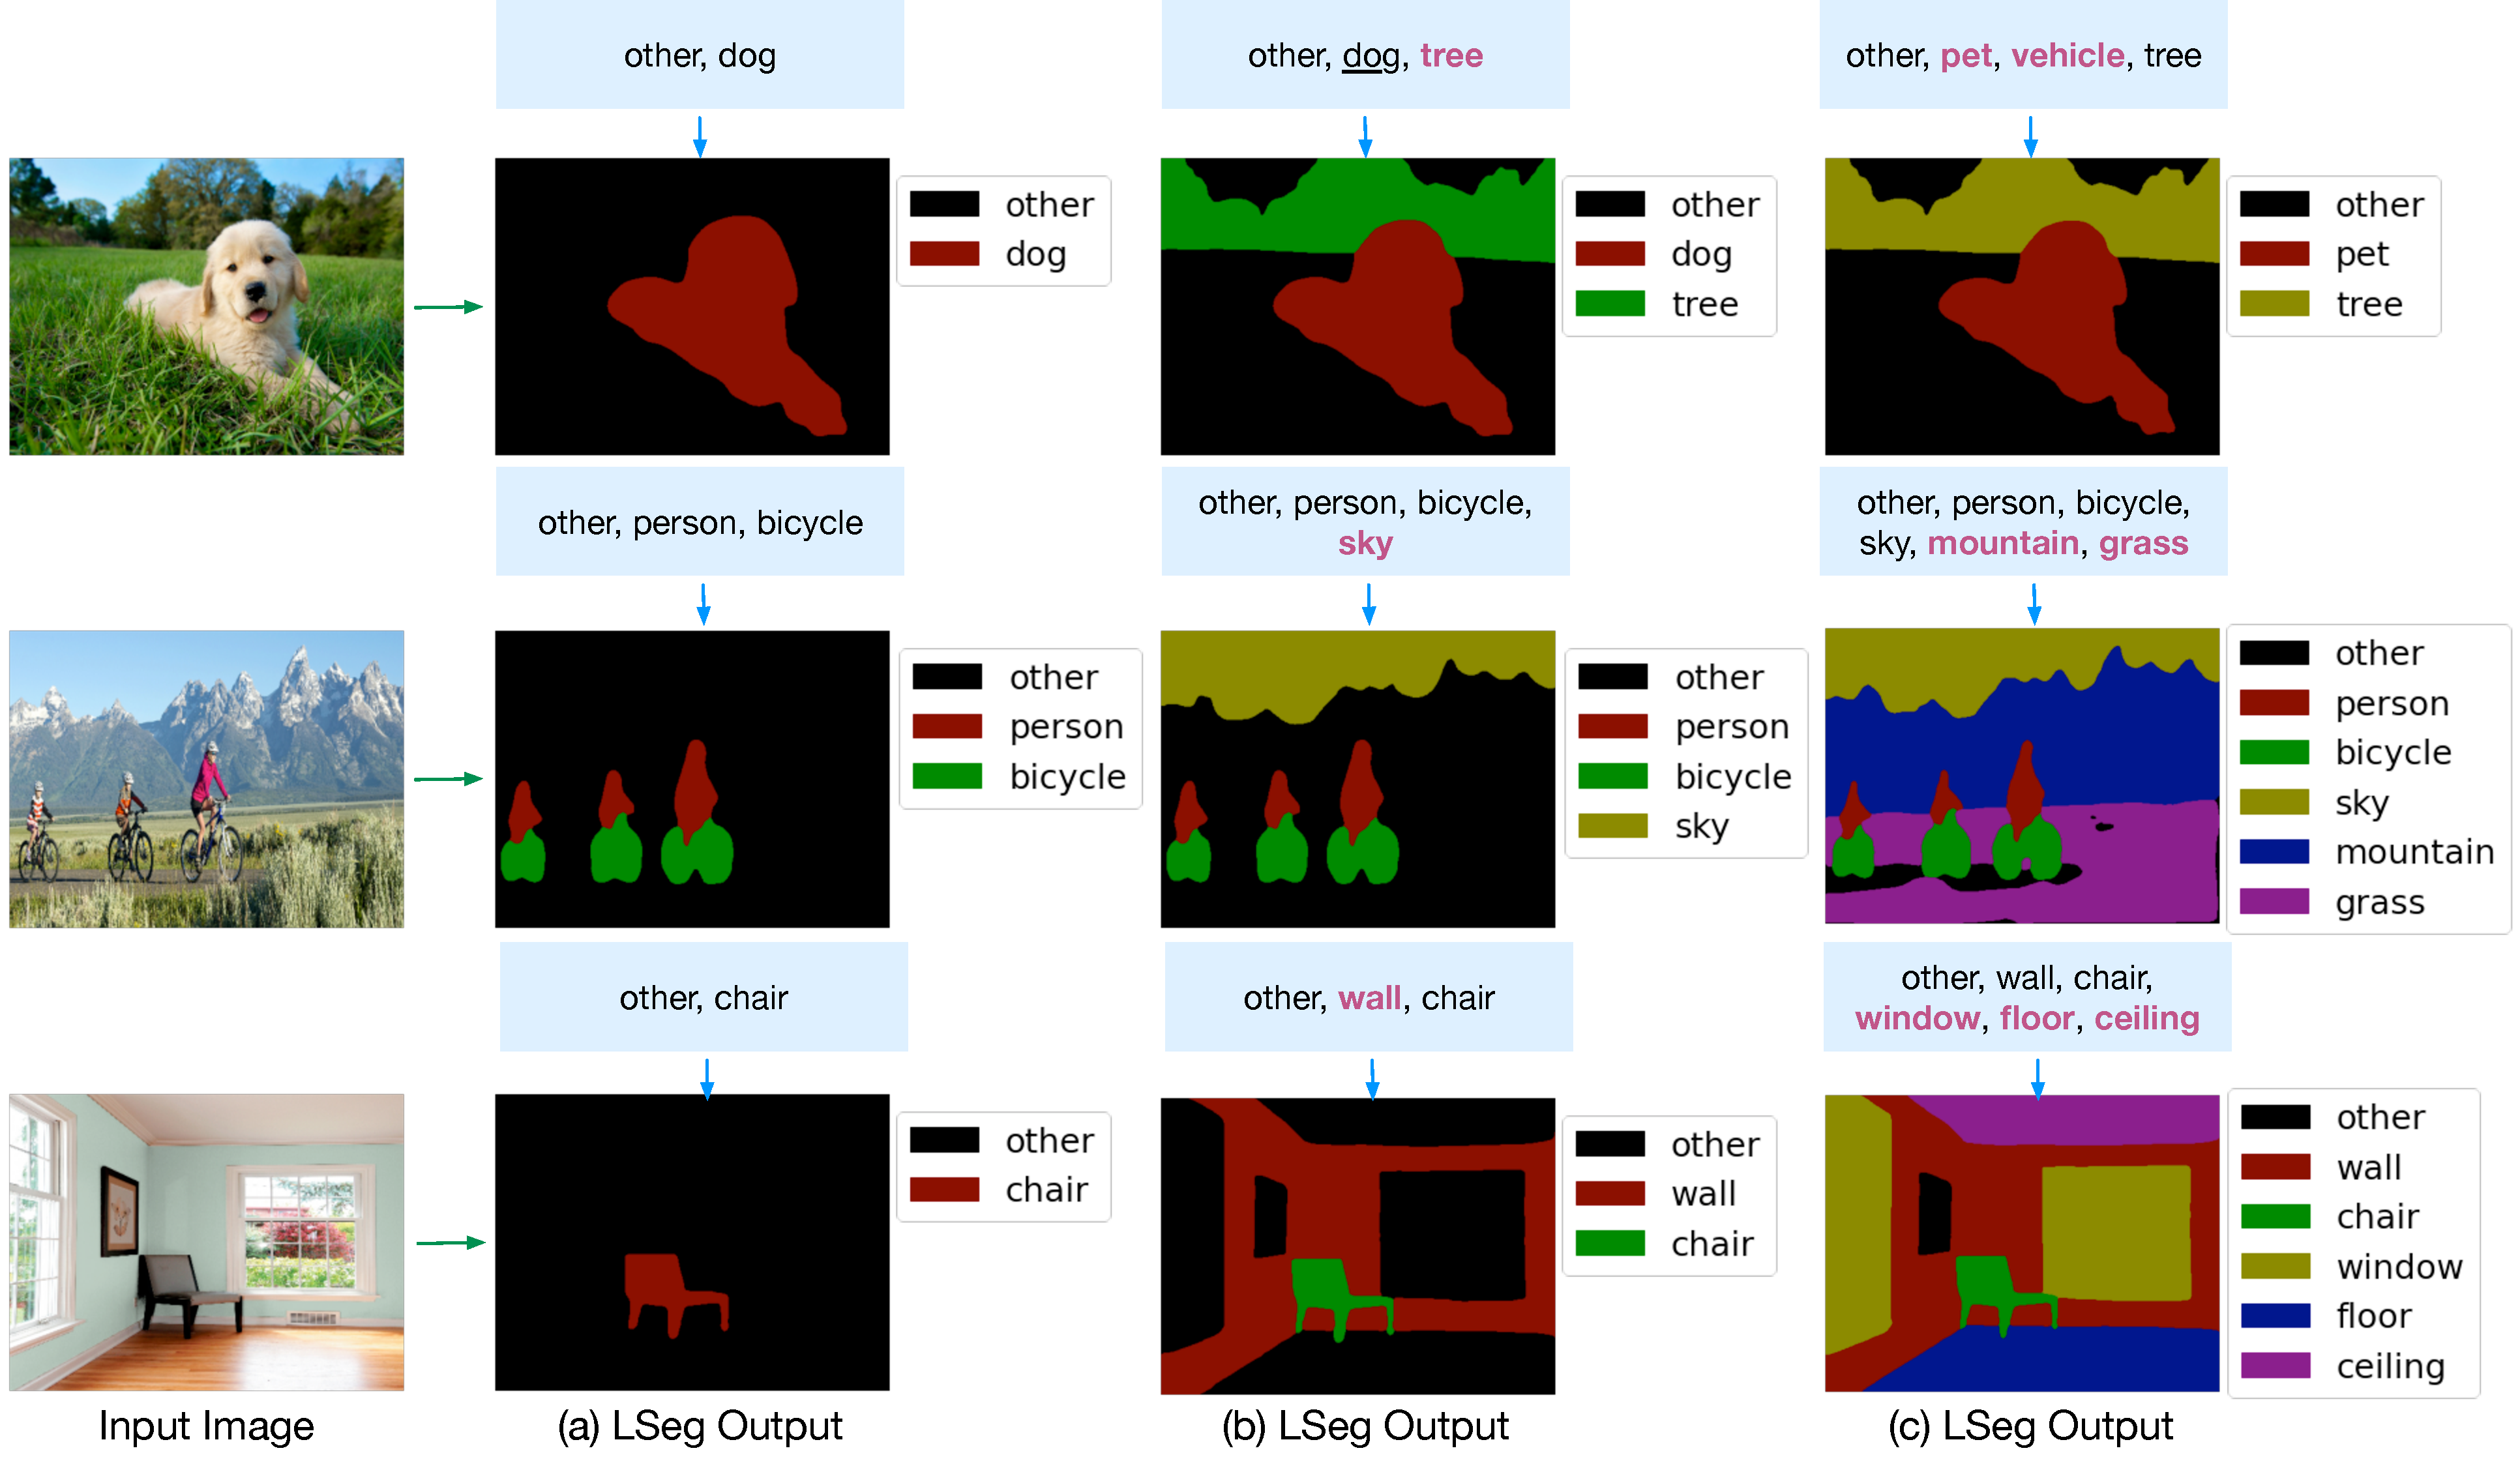
\includegraphics[width=\linewidth]{imgs/exp_random1.pdf}
    \caption{Example results. \methodname{} is able to handle unseen labels as well as label sets of arbitrary length and order. This enables flexible synthesis of zero-shot semantic segmentation models on the fly. From left to right, labels that are removed between runs are \underline{underlined}, whereas labels that are added are marked in \textbf{\textcolor[HTML]{E45E9D}{bold red}}.}
    \label{fig:method_exp1}
    \vspace{-0.2in}
\end{figure}


Our approach enables the synthesis of zero-shot semantic segmentation models on the fly. That is, a user can arbitrarily expand, shrink, or reorder the label set for any image at test time. We further introduce an output module that can spatially regularize the predictions while maintaining this flexibility. We demonstrate several examples of the flexibility of our model in Figure~\ref{fig:method_exp1}. \methodname{} is able to output different segmentation maps based on the provided label set. For instance, in the last row, output (a) recognizes the chair and identifies all non-chair objects as ``other'' since these are the only two labels provided to the model. When labels are added, as in (b) and (c), the model is able to successfully segment other objects with the expanded label set.

We conduct quantitative evaluation on a variety of  zero- and few-shot semantic segmentation tasks. Our approach outperforms existing methods in zero-shot settings and is competitive  across multiple few-shot  benchmarks. Unlike the state-of-the-art baselines we compare to, our approach does not require additional training samples. Our experiments also show that introducing the text embeddings incurs only a negligible loss in performance when compared to standard fixed-label segmentation methods.
